\documentclass[12pt,letterpaper]{hmcpset}
\usepackage[margin=1in]{geometry}
\usepackage{graphicx}
\usepackage{amsmath,amssymb}
\usepackage{enumerate}
\usepackage{hyperref}
\usepackage{parskip}
\usepackage{fourier}

% Theorems
\usepackage{amsthm}
\renewcommand\qedsymbol{$\blacksquare$}
\makeatletter
\@ifclassloaded{article}{
    \newtheorem{definition}{Definition}[section]
    \newtheorem{example}{Example}[section]
    \newtheorem{theorem}{Theorem}[section]
    \newtheorem{corollary}{Corollary}[theorem]
    \newtheorem{lemma}{Lemma}[theorem]
}{
}
\makeatother

% Random Stuff
\setlength\unitlength{1mm}

\newcommand{\insertfig}[3]{
\begin{figure}[htbp]\begin{center}\begin{picture}(120,90)
\put(0,-5){\includegraphics[width=12cm,height=9cm,clip=]{#1.eps}}\end{picture}\end{center}
\caption{#2}\label{#3}\end{figure}}

\newcommand{\insertxfig}[4]{
\begin{figure}[htbp]
\begin{center}
\leavevmode \centerline{\resizebox{#4\textwidth}{!}{\input
#1.pstex_t}}
\caption{#2} \label{#3}
\end{center}
\end{figure}}

\long\def\comment#1{}

\newcommand\norm[1]{\left\lVert#1\right\rVert}
\DeclareMathOperator*{\argmin}{arg\,min}
\DeclareMathOperator*{\argmax}{arg\,max}

% bb font symbols
\newfont{\bbb}{msbm10 scaled 700}
\newcommand{\CCC}{\mbox{\bbb C}}

\newfont{\bbf}{msbm10 scaled 1100}
\newcommand{\CC}{\mbox{\bbf C}}
\newcommand{\PP}{\mbox{\bbf P}}
\newcommand{\RR}{\mbox{\bbf R}}
\newcommand{\QQ}{\mbox{\bbf Q}}
\newcommand{\ZZ}{\mbox{\bbf Z}}
\renewcommand{\SS}{\mbox{\bbf S}}
\newcommand{\FF}{\mbox{\bbf F}}
\newcommand{\GG}{\mbox{\bbf G}}
\newcommand{\EE}{\mbox{\bbf E}}
\newcommand{\NN}{\mbox{\bbf N}}
\newcommand{\KK}{\mbox{\bbf K}}
\newcommand{\KL}{\mbox{\bbf KL}}

% Vectors
\renewcommand{\aa}{{\bf a}}
\newcommand{\bb}{{\bf b}}
\newcommand{\cc}{{\bf c}}
\newcommand{\dd}{{\bf d}}
\newcommand{\ee}{{\bf e}}
\newcommand{\ff}{{\bf f}}
\renewcommand{\gg}{{\bf g}}
\newcommand{\hh}{{\bf h}}
\newcommand{\ii}{{\bf i}}
\newcommand{\jj}{{\bf j}}
\newcommand{\kk}{{\bf k}}
\renewcommand{\ll}{{\bf l}}
\newcommand{\mm}{{\bf m}}
\newcommand{\nn}{{\bf n}}
\newcommand{\oo}{{\bf o}}
\newcommand{\pp}{{\bf p}}
\newcommand{\qq}{{\bf q}}
\newcommand{\rr}{{\bf r}}
\renewcommand{\ss}{{\bf s}}
\renewcommand{\tt}{{\bf t}}
\newcommand{\uu}{{\bf u}}
\newcommand{\ww}{{\bf w}}
\newcommand{\vv}{{\bf v}}
\newcommand{\xx}{{\bf x}}
\newcommand{\yy}{{\bf y}}
\newcommand{\zz}{{\bf z}}
\newcommand{\0}{{\bf 0}}
\newcommand{\1}{{\bf 1}}

% Matrices
\newcommand{\Ab}{{\bf A}}
\newcommand{\Bb}{{\bf B}}
\newcommand{\Cb}{{\bf C}}
\newcommand{\Db}{{\bf D}}
\newcommand{\Eb}{{\bf E}}
\newcommand{\Fb}{{\bf F}}
\newcommand{\Gb}{{\bf G}}
\newcommand{\Hb}{{\bf H}}
\newcommand{\Ib}{{\bf I}}
\newcommand{\Jb}{{\bf J}}
\newcommand{\Kb}{{\bf K}}
\newcommand{\Lb}{{\bf L}}
\newcommand{\Mb}{{\bf M}}
\newcommand{\Nb}{{\bf N}}
\newcommand{\Ob}{{\bf O}}
\newcommand{\Pb}{{\bf P}}
\newcommand{\Qb}{{\bf Q}}
\newcommand{\Rb}{{\bf R}}
\newcommand{\Sb}{{\bf S}}
\newcommand{\Tb}{{\bf T}}
\newcommand{\Ub}{{\bf U}}
\newcommand{\Wb}{{\bf W}}
\newcommand{\Vb}{{\bf V}}
\newcommand{\Xb}{{\bf X}}
\newcommand{\Yb}{{\bf Y}}
\newcommand{\Zb}{{\bf Z}}

% Calligraphic
\newcommand{\Ac}{{\cal A}}
\newcommand{\Bc}{{\cal B}}
\newcommand{\Cc}{{\cal C}}
\newcommand{\Dc}{{\cal D}}
\newcommand{\Ec}{{\cal E}}
\newcommand{\Fc}{{\cal F}}
\newcommand{\Gc}{{\cal G}}
\newcommand{\Hc}{{\cal H}}
\newcommand{\Ic}{{\cal I}}
\newcommand{\Jc}{{\cal J}}
\newcommand{\Kc}{{\cal K}}
\newcommand{\Lc}{{\cal L}}
\newcommand{\Mc}{{\cal M}}
\newcommand{\Nc}{{\cal N}}
\newcommand{\Oc}{{\cal O}}
\newcommand{\Pc}{{\cal P}}
\newcommand{\Qc}{{\cal Q}}
\newcommand{\Rc}{{\cal R}}
\newcommand{\Sc}{{\cal S}}
\newcommand{\Tc}{{\cal T}}
\newcommand{\Uc}{{\cal U}}
\newcommand{\Wc}{{\cal W}}
\newcommand{\Vc}{{\cal V}}
\newcommand{\Xc}{{\cal X}}
\newcommand{\Yc}{{\cal Y}}
\newcommand{\Zc}{{\cal Z}}

% Bold greek letters
\newcommand{\alphab}{\hbox{\boldmath$\alpha$}}
\newcommand{\betab}{\hbox{\boldmath$\beta$}}
\newcommand{\gammab}{\hbox{\boldmath$\gamma$}}
\newcommand{\deltab}{\hbox{\boldmath$\delta$}}
\newcommand{\etab}{\hbox{\boldmath$\eta$}}
\newcommand{\lambdab}{\hbox{\boldmath$\lambda$}}
\newcommand{\epsilonb}{\hbox{\boldmath$\epsilon$}}
\newcommand{\nub}{\hbox{\boldmath$\nu$}}
\newcommand{\mub}{\hbox{\boldmath$\mu$}}
\newcommand{\zetab}{\hbox{\boldmath$\zeta$}}
\newcommand{\phib}{\hbox{\boldmath$\phi$}}
\newcommand{\psib}{\hbox{\boldmath$\psi$}}
\newcommand{\thetab}{\hbox{\boldmath$\theta$}}
\newcommand{\taub}{\hbox{\boldmath$\tau$}}
\newcommand{\omegab}{\hbox{\boldmath$\omega$}}
\newcommand{\xib}{\hbox{\boldmath$\xi$}}
\newcommand{\sigmab}{\hbox{\boldmath$\sigma$}}
\newcommand{\pib}{\hbox{\boldmath$\pi$}}
\newcommand{\rhob}{\hbox{\boldmath$\rho$}}

\newcommand{\Gammab}{\hbox{\boldmath$\Gamma$}}
\newcommand{\Lambdab}{\hbox{\boldmath$\Lambda$}}
\newcommand{\Deltab}{\hbox{\boldmath$\Delta$}}
\newcommand{\Sigmab}{\hbox{\boldmath$\Sigma$}}
\newcommand{\Phib}{\hbox{\boldmath$\Phi$}}
\newcommand{\Pib}{\hbox{\boldmath$\Pi$}}
\newcommand{\Psib}{\hbox{\boldmath$\Psi$}}
\newcommand{\Thetab}{\hbox{\boldmath$\Theta$}}
\newcommand{\Omegab}{\hbox{\boldmath$\Omega$}}
\newcommand{\Xib}{\hbox{\boldmath$\Xi$}}

% mixed symbols
\newcommand{\sinc}{{\hbox{sinc}}}
\newcommand{\diag}{{\hbox{diag}}}
\renewcommand{\det}{{\hbox{det}}}
% \newcommand{\trace}{{\hbox{tr}}}
% \newcommand{\tr}{\trace}
\newcommand{\sign}{{\hbox{sign}}}
\renewcommand{\arg}{{\hbox{arg}}}
\newcommand{\var}{{\hbox{var}}}
\newcommand{\cov}{{\hbox{cov}}}
\renewcommand{\Re}{{\rm Re}}
\renewcommand{\Im}{{\rm Im}}
\newcommand{\eqdef}{\stackrel{\Delta}{=}}
\newcommand{\defines}{{\,\,\stackrel{\scriptscriptstyle \bigtriangleup}{=}\,\,}}
\newcommand{\<}{\left\langle}
\renewcommand{\>}{\right\rangle}
\newcommand{\Psf}{{\sf P}}
\newcommand{\T}{\top}
\newcommand{\m}[1]{\begin{bmatrix} #1 \end{bmatrix}}

\usepackage{physics}
% info for header block in upper right hand corner
\name{Colin Adams} 
\class{Math189R SU20}
\assignment{Homework 2}
\duedate{June 2020}

\begin{document}

Feel free to work with other students, but make sure you write up the homework
and code on your own (no copying homework \textit{or} code; no pair programming).
Feel free to ask students or instructors for help debugging code or whatever else,
though.
\newline
\newline
The starter files can be found under the Resource tab on course website. The graphs for problem 3 generated by the sample solution could be found in the corresponding zipfile. These graphs only serve as references to your implementation. You should generate your own graphs for submission. Please print out all the graphs generated by your own code and submit them together with the written part, and make sure you upload the code to your Github repository.\\

\begin{problem}[1]
	(\textbf{Murphy 8.3}) Gradient and Hessian of the log-likelihood for
	logistic regression.
	\begin{enumerate}[(a)]
		\item Let $\sigma(x) = \frac{1}{1 + e^{-x}}$ be the sigmoid function. Show that
		\[
		\sigma'(x) = \sigma(x)\left[1 - \sigma(x)\right].
		\]
		\item Using the previous result and the chain rule of calculus, derive an
		expression for the gradient of the log likelihood for logistic regression.
		\item The Hessian can be written as $\Hb=\Xb^\T\Sb\Xb$ where $\Sb =
		\diag(\mu_1(1-\mu_1), \dots, \mu_n(1-\mu_n))$. Derive this and show that
		$\Hb \succeq 0$ ($A \succeq 0$ means that $A$ is positive semidefinite).\\
	\end{enumerate} 

\textit{Hint:} Use the \textbf{negative} log-likelihood of logistic regression for this problem.
\end{problem}
\begin{solution}
	\begin{enumerate}[(a)]
		\item Note that 
		\begin{align*}
			1 - \sigma(x) = \frac{e^{-x}}{1+ e^{-x}} \qq{and} \sigma'(x) = \frac{e^{-x}}{\left(1 + e^{-x}\right)^2},
		\end{align*}
		which makes it easy to see that
		\begin{align*}
			\sigma'(x) = \frac{e^{-x}}{\left(1 + e^{-x}\right)^2} = \frac{e^{-x}}{1+ e^{-x}} \frac{1}{1+ e^{-x}} = \sigma(x) (1 - \sigma(x)).
		\end{align*}


		\item Okay, so if we use the negative log-likelihood of the logistic regression, we have
		\begin{align*}
			{\rm NLL} = - \sum_i \qty[ y_i \ln \sigma(\vb w \vdot \vb x_i) + (1 - y_i) \ln(1 - \sigma(\vb w \vdot \vb x_i))]
		\end{align*}
		and if we take the gradient with respect to $\vb w$ is given by 
		\begin{align*}
			\grad_{\vb w} {\rm NLL} &= - \sum_i \grad_{\vb w} \qty[ y_i \ln \sigma(\vb w \vdot \vb x_i) + (1 - y_i) \ln(1 - \sigma(\vb w \vdot \vb x_i))] \\
			&= -\sum_i \qty[ y_i \frac{\sigma'(\vb w \vdot \vb x_i)}{\sigma(\vb w \vdot \vb x_i)}\vb x_i 
			-
			(1 - y_i) \frac{\sigma'(\vb w \vdot \vb x_i)}{1 - \sigma(\vb w \vdot \vb x_i)} \vb x_i
			] \\
			&= -\sum_i \qty[ y_i (1 - \sigma(\vb w \vdot \vb x_i))\vb x_i 
			-
			(1 - y_i) \sigma(\vb w \vdot \vb x_i)\vb x_i
			] &\qq{(result of (a))} \\
			&= \sum_i \qty[ \sigma(\vb w \vdot \vb x_i) - y_i]\vb x_i
		\end{align*}
		which can be rewritten in a more compact matrix form as
		\begin{align*}
			\grad_{\vb w} {\rm NLL} = \vb X^T (\boldsymbol\mu - \vb y) \qq{where} \mub = \sigma(\vb X \vb w ).
		\end{align*}

		\item The Hessian $\vb H$ is the gradient of the gradient (transposed) and so 
		\begin{align*}
			\vb H &= \grad_{\vb w} \qty( \vb X^T (\boldsymbol\mu - \vb y) )^T \\
			&= \grad_{\vb w} \qty( (\boldsymbol\mu  - \vb y)^T \vb X) \\
		    &= \qty(\sum_i \grad_{\vb w}\qty[ \sigma(\vb w \vdot \vb x_i)]\vb x_i) \vb X \\
		    &= \qty(\sum_i \sigma(\vb w \vdot \vb x_i)(1 - \sigma(\vb w \vdot \vb x_i)) \vb x_i \vb x_i^T )\vb X \\
		    &= \qty(\sum_i \mu_i (1 - \mu_i) \vb x_i \vb x_i^T )\vb X \\
		    &= \vb X^T \diag(\mu_i(1-\mu_i)) \vb X \\
		    &=  \vb X^T \vb S \vb X \qq{ where } \vb S \equiv \diag(\mu_i(1-\mu_i))
		\end{align*}
		which is what we were hoping to get. Phew. Now we need to show that $\vb H$ is positive semidefinite, which means $\braket{ \vb v}{\vb H\vb v} \ge 0$ for any nonzero $\vb v$. A way to do this is to look at the components. So 
		\begin{align*}
			H_{ij} = x_i^2 x_j^2 \mu_i (1 - \mu_i) \delta_{ij} \qq{where $\delta_{ij}$ is the Kronecker delta function}
		\end{align*}
		and so---using the Einstein summation convention---we find $\braket{\vb v}{\vb H \vb v} $ then
		\begin{align*}
			\braket{ \vb v}{\vb H \vb v} &= v_i H_{ij} v_j \\
			&= v_i ( x_j x_i \mu_i(1 - \mu_i) v_j \delta_{i j} x_i x_j) v_j \\
			&= v_i v_j x_i^2 x_j^2 \mu_i(1 - \mu_i)  \delta_{ij} \\
			&= v_i^2 x_i^4\mu_i(1 - \mu_i) 
		\end{align*}
		and since $\sum_i (v_i x_i^2)^2 \ge 0$ for all $v_i, x_i \in \mathbb R,$ we only need to really care about the $\mu_i(1 - \mu_i)$ term. Since $0<\mu_i<1$ then $\mu_i(1 - \mu_i)$ is also greater than zero. Therefore, $\braket{\vb v}{\vb H \vb v} \ge 0$ and so $\vb H$ is positive, semi-definite, i.e.\ $\vb H \succeq 0.$
	\end{enumerate}
\end{solution}
\newpage

\begin{problem}[2]
	(\textbf{Murphy 2.11})
	Derive the normalization constant ($Z$) for a one dimensional
	zero-mean Gaussian
	\[
	\PP(x; \sigma^2) = \frac{1}{Z}\exp\left(-\frac{x^2}{2\sigma^2}\right)
	\]
	such that $\PP(x; \sigma^2)$ becomes a valid density.
\end{problem}
\begin{solution}
	I'm just going to call $\PP$ with the easier-to-type $p$ if that's okay. Well, we need to use the fact that
	\begin{align*}
		\int p(x) \dd{x} = 1.
	\end{align*}
	In our case
	\begin{align*}
		p(x)= \frac{1}{Z}\exp\left(-\frac{x^2}{2\sigma^2}\right)
	\end{align*}
	so 
	\begin{align*}
		1 = \frac{1}{Z} \int_{-\infty}^\infty \exp(-\frac{x^2}{2\sigma^2}) \dd{x}.
	\end{align*}
	Unfortuntately, this is a hard integral to solve, so we might as well make it twice as hard. If we let 
	\begin{align*}
		I = \int_{-\infty}^\infty \exp(-\frac{x^2}{2\sigma^2}) \dd{x}
	\end{align*}
	then
	\begin{align*}
		I^2 &= \int_{-\infty}^\infty \exp(-\frac{x^2}{2\sigma^2}) \dd{x} \int_{-\infty}^\infty \exp(-\frac{y^2}{2\sigma^2}) \dd{y} \\
		&= \int_{-\infty}^\infty\int_{-\infty}^\infty \exp(-\frac{x^2 + y^2}{2\sigma^2}) \dd{x} \dd{y}.
	\end{align*}
	We can evaluate this using polar coordinates, so 
	\begin{align*}
		I^2 &= \int_0^{2\pi} \int_0^\infty \exp(-r^2/2\sigma^2) r \dd{r} \dd{\theta} \\
		&= 2\pi\sigma^2 \int_{-\infty}^0 \exp(u) \dd{u}   &\qq{(using a $u$-sub.\ with $u = -r^2/2\sigma^2$.)} \\
		&= 2\pi\sigma^2 
	\end{align*}
	which implies $I = \sqrt{2\pi}\sigma = 1/Z.$ And, finally, $Z = 1/\sqrt{2\pi}\sigma.$ Special shout out to Prof.\ Saeta for showing us how to solve this like three years ago now. His unparalleled sass allowed me to remember exactly what he did to solve this.
	\vfill
\end{solution}
\newpage

\begin{problem}[3]
(\textbf{regression}). In this problem, we will use the online news popularity dataset to set up a model for linear regression. In the starter code, we have already parsed the data for you. However, you might need internet connection to access the data and therefore successfully run the starter code.
\newline \newline
We split the csv file into a training and test set with
the first two thirds of the data in the training set and the rest for testing.
Of the testing data, we split the first half into a `validation set' (used
to optimize hyperparameters while leaving your testing data pristine) and
the remaining half as your test set.
We will use this data for the remainder of the problem. The goal of this data
is to predict the \textbf{log} number of shares a news article will have given the other
features.
\newline \newline
\begin{enumerate}[(a)]
	\item (\textbf{math}) Show that the maximum a posteriori problem for
	linear regression with a zero-mean Gaussian prior $\PP(\ww) = \prod_j
	\Nc(w_j | 0, \tau^2)$ on the weights,
	\[
	\argmax_\ww \sum_{i=1}^N \log\Nc(y_i | w_0 + \ww^\T\xx_i, \sigma^2) + \sum_{j=1}^D \log\Nc(w_j | 0, \tau^2)
	\]
	is equivalent to the ridge regression problem
	\[
	\argmin \frac{1}{N}\sum_{i=1}^N (y_i - (w_0 + \ww^\T\xx_i))^2 + \lambda ||\ww||_2^2
	\]
	with $\lambda = \sigma^2 / \tau^2$.
	\newline
	\item (\textbf{math}) Find a closed form solution $\xx^\star$ to the ridge regression
	problem:
	\[
	\text{minimize: } ||A\xx - \bb||_2^2 + ||\Gamma\xx||_2^2.
	\]
	
	\item
	(\textbf{implementation}) Attempt to predict the $\log\text{shares}$ using ridge
regression from the previous problem solution. Make sure you include a bias
term and \textit{don't regularize the bias term}.
Find the optimal regularization parameter $\lambda$
from the validation set. Plot both $\lambda$ versus the validation RMSE (you should have
tried at least 150 parameter settings randomly chosen between 0.0 and 150.0 because
the dataset is small)
and $\lambda$ versus $||\thetab^\star||_2$ where $\thetab$ is your weight vector.
What is the final RMSE on the test set with the optimal $\lambda^\star$?\\
\newline
(continued on the following pages)
\end{enumerate}
\end{problem}
\begin{solution}
	\vfill
\end{solution}
\newpage

\begin{problem}[3 (continued)]
\begin{enumerate}[(a)]
	\setcounter{enumi}{3}
\item (\textbf{math}) Consider regularized linear regression where we pull the
basis term out of the feature vectors. That is, instead of computing $\hat\yy
= \thetab^\T\xx$ with $\xx_0 = 1$, we compute $\hat\yy = \thetab^\T\xx + b$.
This corresponds to solving the optimization problem
\[
\text{minimize: } ||A\xx + b\1 - \yy||_2^2 + ||\Gamma\xx||_2^2.
\]
Solve for the optimal $\xx^\star$ explicitly. Use this close form to compute the
bias term for the previous problem (with the same regularization strategy). Make
sure it is the same.
\newline
\item (\textbf{implementation}) We can also compute the solution to the least squares
problem using gradient descent. Consider the same bias-relocated objective
\[
\text{minimize: } f = ||A\xx + b\1 - \yy||_2^2 + ||\Gamma\xx||_2^2.
\]
Compute the gradients and run gradient descent. Plot the $\ell_2$ norm
between the optimal $(\xx^\star, b^\star)$ vector you computed in closed form
and the iterates generated by gradient descent. Hint: your plot should move
down and to the left and approach zero as the number of iterations increases. If
it doesn't, try decreasing the learning rate.
\end{enumerate}
\end{problem}
\begin{solution}
		\begin{enumerate}[(a)]
		\item Well, if we are looking for $\vb w$ such that \[\sum_{i=1}^N \log\Nc(y_i | w_0 + \ww^\T\xx_i, \sigma^2) + \sum_{j=1}^D \log\Nc(w_j | 0, \tau^2)\] is maximized, let's plug in the normal distributions and ignore any constant terms, then we can do a little rearranging to see 
		\begin{align*}
			{\rm answer} &=\argmax_\ww \sum_{i=1}^N \log\Nc(y_i | w_0 + \ww^\T\xx_i, \sigma^2) + \sum_{j=1}^D \log\Nc(w_j | 0, \tau^2) \\ &= 
			\argmax_\ww \sum_i^N \frac{-\qty(y_i - (w_0 + \ww \vdot \xx_i))^2}{2\sigma^2} - \sum_i^D - \frac{w_i^2}{2\tau^2} \\
			&= \argmin_\ww \sum_i^N \frac{\qty(y_i - (w_0 + \ww \vdot \xx_i))^2}{2\sigma^2} + \sum_i^D \frac{w_i^2}{2\tau^2} \\
			&= \argmin_\ww \sum_i^N \frac{\qty(y_i - (w_0 + \ww \vdot \xx_i))^2}{2\sigma^2} + \frac{1}{2\tau^2} \norm{\ww}^2.
		\end{align*}
		Since we can multiply the function by some constant without affecting where the maximum $\ww$ occurs, we can get
		\begin{align*}
			{\rm answer}= \argmin_\ww \sum_i^N \qty(y_i - (w_0 + \ww \vdot \xx_i))^2 + \frac{\sigma^2}{\tau^2} \norm{\ww}^2.
		\end{align*}
		We can also just scale the first term without changing where $\ww$ maximizes the function, so
		\begin{align*}
			{\rm answer} = \argmin_\ww \frac1N\sum_i^N \qty(y_i - (w_0 + \ww \vdot \xx_i))^2 + \frac{\sigma^2}{\tau^2} \norm{\ww}^2
		\end{align*}
		as desired. I'm sorry for the clunky notation.


		\item Well, I guess we should probably rewrite $\norm{\vb A \vb x - \vb b}^2$ and $\norm{\Gamma \vb x}^2$. Since
		\begin{align*}
			\norm{\Gamma \vb x}^2 = \vb x^T \Gamma^T \Gamma \vb x \qq{and} \norm{\vb A \vb x - \vb b}^2 &= \qty(\vb A \vb x - \vb b)^T \qty(\vb A \vb x - \vb b) \\
			&= \vb x^T \vb A^T \vb A \vb x - 2 \vb x^T \vb A^T \vb b + \vb b^T \vb b 
		\end{align*}
		then we can take the gradient with respect to $\vb x$ and get
		\begin{align*}
			\dv{\vb x}\qty(\norm{\vb A \vb x - \vb b}^2 + \norm{\Gamma \vb x}^2 ) &= \dv{\vb x}\qty(\vb x^T \vb A^T \vb A \vb x - 2 \vb x^T \vb A^T \vb b + \vb b^T \vb b ) + \dv{\vb x}\qty(\vb x^T \Gamma^T \Gamma \vb x )\\
			&= 2 \qty(\vb A^T \vb A \vb x - \vb A^T \vb b + \Gamma^T \Gamma \vb x).
		\end{align*}
		We should probably set this to zero to find a critical point (presumably a minimum since there's no bound to how poorly you can do) and solve for $\vb x$ so
		\begin{align*}
		\vb A^T \vb A \vb x - \vb A^T \vb b + \Gamma^T \Gamma \vb x &= 0 \\
		\Rightarrow 
		\qty(\vb A^T \vb A  + \Gamma^T \Gamma )\vb x &=  \vb A^T \vb b 
		\end{align*}
		And thus, 
		\begin{align*}
			\vb x = \qty(\vb A^T \vb A  + \Gamma^T \Gamma )^{-1}\vb A^T \vb b .
		\end{align*}

		\item We plot $\lambda$ vs.\ the root mean square error as well as $\norm{\thetab}$ below. 
		\begin{center}
			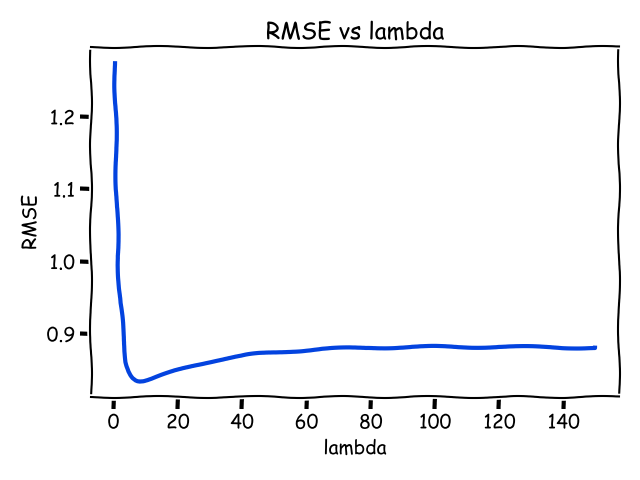
\includegraphics[width = 3.in]{hw2_starter_files/RMSE_vs_lambda.png}
			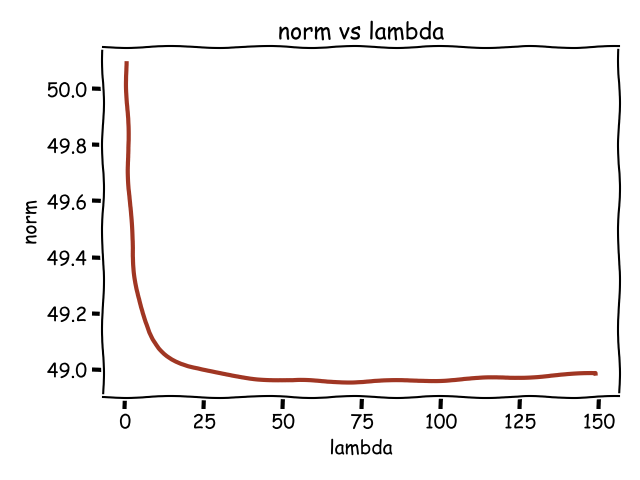
\includegraphics[width = 3.in]{hw2_starter_files/norm_vs_lambda.png}
		\end{center}

		The optimal regularization value was $\lambda = 8.4493$ with a root mean square error of 0.8340 on the validation set and 0.8628 on the test set.

		\item Well, we're looking to minimize \[ 
		||A\xx + b\1 - \yy||_2^2 + ||\Gamma\xx||_2^2 = 
			\vb x^T \vb A^T \vb A \vb x - 2 \vb x^T \vb A^T \vb b 
			%
			+2 \vb b^T \vb A \vb x - 2\vb b^T \vb y
			%
			+ \vb b^T \vb b + \vb x^T \Gamma^T \Gamma \vb x
		\] where $\vb b = b \vb 1$ so we should probably take a gradient
		\begin{align*}
		 	\dv{\vb x}\qty (||A\xx + b\1 - \yy||_2^2 + ||\Gamma\xx||_2^2) &= \dv{\vb x}\qty(\vb x^T \vb A^T \vb A \vb x - 2 \vb x^T \vb A^T \vb b 
			%
			+2 \vb b \vb A \vb x - 2\vb b^T \vb y
			%
			+ \vb b^T \vb b + \vb x^T \Gamma^T \Gamma \vb x + 2 \vb y^T \vb A \vb x + \vb y^T \vb y) \\
			%
			&= 2 \qty(\vb A^T \vb A \vb x - \vb A^T \vb b + \Gamma^T \Gamma \vb x + \vb A^T \vb y) 
		 \end{align*} 
		 which we set equal to zero and solve for $\vb x$, so 
		 \begin{align*}
		 	&\vb A^T(\vb b - \vb y)  = (\vb A^T \vb A + \Gamma^T \Gamma)\vb x 
		 	&\Rightarrow \vb x = (\vb A^T \vb A + \Gamma^T \Gamma)^{-1}\vb A^T(\vb b - \vb y).
		 \end{align*}
		 which isn't super helpful, I suppose without $\vb b.$ Sad. I guess, doing the same thing of taking the gradient of the norm terms with respect to $\vb b$---or really $b$ where $\vb b = b \vb 1$---gives us
		 \begin{align*}
		 	\dv{b}\qty( \vb x^T \vb A^T \vb A \vb x - 2 \vb x^T \vb A^T \vb b 
			%
			+2 \vb b^T \vb A \vb x - 2\vb b^T \vb y
			%
			+ \vb b^T \vb b + \vb x^T \Gamma^T \Gamma \vb x ) 
			 &= 2\qty( b \vb 1^T \vb 1 - \vb 1^T \vb y + \vb 1^T \vb A \vb x )
		 \end{align*}
		 which we set to zero to find 
		 \begin{align*}
		 	 b = \frac1n \vb 1^T(\vb y - \vb A \vb x)
		 \end{align*}
		 which is disappointing because I need to plug it into our $\vb x$ equation and resolve for $\vb x$. FML.  So 
		 \begin{align*}
		 	\vb x = (\vb A^T \vb A + \Gamma^T \Gamma)^{-1} \vb A^T \qty( \frac1n \vb 1^T(\vb y - \vb A \vb x) \vb 1 - \vb y),
		 \end{align*}
		 which can be rearranged to give 
		 \begin{align*}
		(\vb A^T \vb A + \Gamma^T \Gamma) \vb x &= \vb A^T \qty( \frac1n \vb 1^T(\vb y - \vb A \vb x) \vb 1 - \vb y) \\
		&= \vb A^T \qty( \frac1n \vb 1 \vb 1^T \vb y - \frac1n \vb 1 \vb 1^T \vb A \vb x - \vb y ) \\
		&= \vb A^T  \frac1n \vb 1 \vb 1^T \vb y - \vb A^T \frac1n \vb 1 \vb 1^T \vb A \vb x - \vb A^T \vb y \\
		 \qty(\vb A^T \vb A + \Gamma^T \Gamma + \vb A^T \frac1n \vb 1 \vb 1^T) \vb A  \vb x &= \vb A^T  \frac1n \vb 1 \vb 1^T \vb y - \vb A^T \vb y \\
		\qty(\vb A^T ( \vb I - \frac1n \vb 1 \vb 1^T) \vb A + \Gamma^T \Gamma) \vb x &= \vb A^T (\vb I - \frac1n \vb 1 \vb 1^T) \vb A \vb y  
		 \end{align*}
		 which tells us that
		 \begin{align*}
		 	\vb x = \qty[\vb A^T \qty( \vb I - \frac1n \vb 1 \vb 1^T) \vb A + \Gamma^T \Gamma]^{-1} \vb A^T \qty(\vb I - \frac1n \vb 1 \vb 1^T) \vb A \vb y  
		 \end{align*}
		 which is a horribly disgusting---but analytic---answer.


		\item Here is our convergence plot:
		\begin{center}
			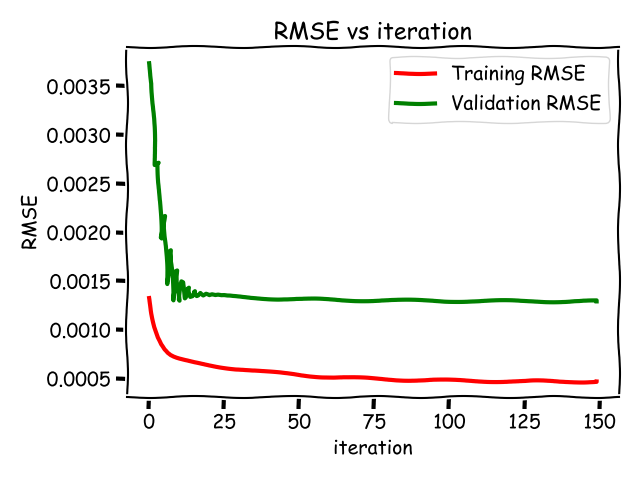
\includegraphics[width = 4in]{hw2_starter_files/convergence.png}
		\end{center}
		The difference between the norms is 080378 and the difference between the biases is 0.15388.
	\end{enumerate}
	\vfill
\end{solution}
\newpage

\end{document}
